\documentclass[a4paper]{article} 
\usepackage{graphicx,amssymb} 
\usepackage{amsmath,bm,bbm}
\usepackage{hyperref}
\usepackage{cite}
\usepackage[left=35mm, right=35mm, top=15mm, bottom=20mm, noheadfoot]{geometry}

\textwidth=15cm \hoffset=-1.2cm 
\textheight=25cm \voffset=2cm 

\pagestyle{empty} 

\date{} 

\def\keywords#1{{\bf Keywords: }{#1}}

\begin{document}
\thispagestyle{empty}

\title{\textbf{Theory of information and computational statistics in signal processing and analysis - Optimized implementations in \texttt{R}}}

\author{Eduarda T. C. Chagas, Alejandro C. Frefry \\ 
	Universidade Federal de Alagoas \\ \\ 
	\tt{etcc@ic.ufal.br}
}

\date{}
\maketitle\thispagestyle{empty} 


\begin{abstract}
A time series consists of a set of data obtained sequentially through observations over a period of time, not precisely partitioned in equal spaces of time, resulting from the operation of a causal system subject to observational noises, where it has as a great differential the dependence and the consequent existence of patterns present among its elements.

Being a solid area in Statistics, the analysis of time series has a wide application in the most diversified areas, such as bank data analysis, vehicular network characterization, seismic data, among many other examples.

There are several ways to perform the analysis of these data, however the vast majority of them are composed of language libraries dedicated to the development of mathematical calculations, which require a minimum knowledge of them. In this way, the project aims to provide a friendly graphical tool with efficient, fast and good numerical quality functionalities that allows an interactive and exploratory analysis of the data of the time series through techniques derived from Information Theory, having as fundamental requirements portability for different operating systems and hardware architectures, and the use of FLOSS (Free / Open Source Software) tools.

In carrying out the process of time series analysis, we have as main objective to determine patterns in the midst of inherent randomness so characteristic, so that it becomes possible the analysis and consequent decision making based on these results.
Based on the Information Theory, specific properties of a
temporal series, contributing to their better study.

Being a time series $\bm x = (x_1, x_2, \dots, x_n)$, by the technique of \textit{simbolização de Bandt \& Pompe}~\cite{PermutationEntropyBandtPompe},
we will transform the data into groups of $N$ values and ordinal patterns, only to analyze their frequency distribution. Therefore, for $N = 3$ and any $i$,
for each $x_i<x_{i+1}<x_{i+2}$ we have a given pattern $\pi_0$ associated. The probability distribution will thus be computed by means of the relative frequency of each of the possible $N!$ Patterns.

Some quantifiers such as entropy, stochastic distance to an equilibrium distribution, and statistical complexity may be extracted from the histogram of the given probability distribution.

Since the Shannon entropy is the metric used to measure the system disorder that gave rise to the $\bm x$ data, we can compute them from $\bm h = (h_1, \dots, h_{N!}$ , the histogram of the proportions of the standard $N!$ observed from the time series $\bm x$.

\begin{equation}
H(\bm h) = \sum_{i=1}^{N!} (-\log h_i) h_i,
\label{eq:Entropia}
\end{equation}

Where we will by convention $-\infty 0=0$.

Through the uniform distribution $\bm u=(1/N!,\dots,1/N!)$ We can also compute the Jensen-Shannon distance, thus being able to measure how close or far the underlying dynamics lie in a process without information.

\begin{equation}
D(\bm h,\bm u) = \sum_{i=1}^{N!} \Big(h_i \log\frac{h_i}{u_i} +
u_i \log\frac{u_i}{p_i}
\Big),
\end{equation}

where $u_i=1/N!$.

We can also calculate its statistical complexity, which seeks to find structures of interaction and dependence between the elements of a given series.

\begin{equation}
C(\bm h, \bm u) = H(\bm h) D(\bm h, \bm u).
\end{equation}

Every time series can be described by a point $(H(\bm h), C(\bm h, \bm u))$ in a compact subset $\mathbbm R^2$: the Entropy-Complexity plane. By means of such a tool it is possible to discover the nature of the series, determining if this is a chaotic, stochastic or deterministic sequence, analyzing its behavior, since these have different dynamics ~\cite{Rosso2007}.

Although only the Shannon entropy and the Jensen-Shannon divergence were cited, the project provides other entropy options ~\cite{salicruetal1993} and stochastic distances ~\cite{StatisticalInferenceBasedonDivergenceMeasures}. With the contribution of our system, analyzes of the underlying dynamics of time series can be enriched by other descriptors, aiding several successful areas using \textit{Bandt \& Pompe symbolization}, for example, in the recognition of patterns of behavior in vehicular networks ~\cite{CharacterizationVehicleBehaviorInformationTheory} and in the discrimination between stochastic and chaotic phenomena ~\cite{DistinguishingNoiseFromChaos}.

\begin{figure}[hbt]
	\centering
	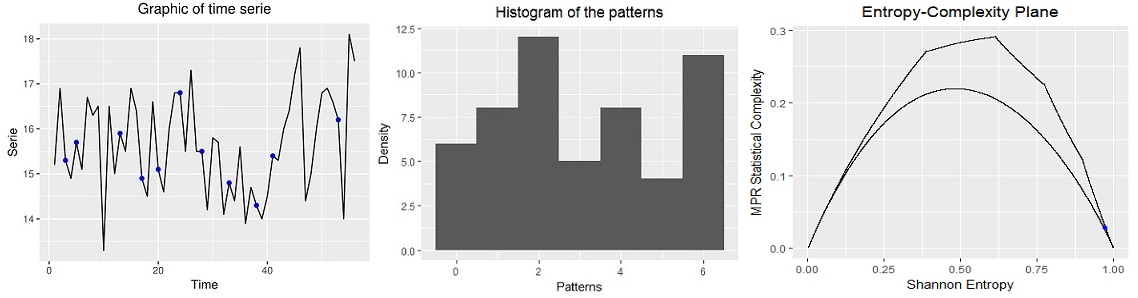
\includegraphics[width=1\columnwidth]{rplot}        
     \caption{Graphical representation of the analysis of a time series of annual production of barley per acre.}
\end{figure}

\end{abstract}

\keywords{Time series, information theory, \texttt R language.}

\bibliographystyle{unsrt}
\bibliography{ref}

\end{document}